%-- Add sections and your outline will be created automatically --%
\section{Tides in the Mediterranean Sea}

% Frame starts a new slide
\begin{frame}
    \frametitle{Tides in the Mediterranean Sea}
\begin{itemize}
\item Tidal modelling is a widely used method for validating free surface implementations.
\item Tides introduced by an astronomical body forcing, and a
\item Co--oscillating boundary tide forcing.
\item This example considers the four main tidal constituents: \mbox{$M_2, \, S_2, \, K_1 \,\, {\rm and} \,\, O_1$}.
\end{itemize}
\end{frame}
%
\begin{frame}
    \frametitle{Tides in the Mediterranean Sea}
\begin{figure}
\centering
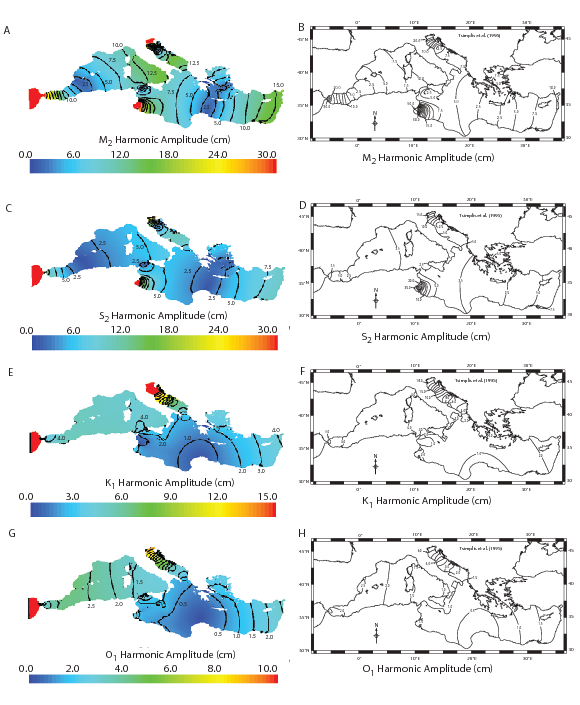
\includegraphics[width=0.9\textwidth, clip = True, trim = 5mm 180mm 0mm 0mm]{./tides_in_the_Mediterranean_Sea/amp.png}
\caption{The $M_2$ tidal harmonic amplitude from (left) Fluidity--ICOM and (right) a high resolution tidal model${}^\dagger$.}
\end{figure}
\footnote{${}^\dagger$ M.~N.~Tsimplis {\it et al.} (1995), J. Geophys. Res. 100 (C8).}
\end{frame}
%

\begin{frame}
    \frametitle{Tides in the Mediterranean Sea}
The amplitude of each of the todal components is considered, and a RMS error of the difference of these to observed tide guage data is calculated.  The locations of these tide guages is shown below.
\begin{figure}
\centering
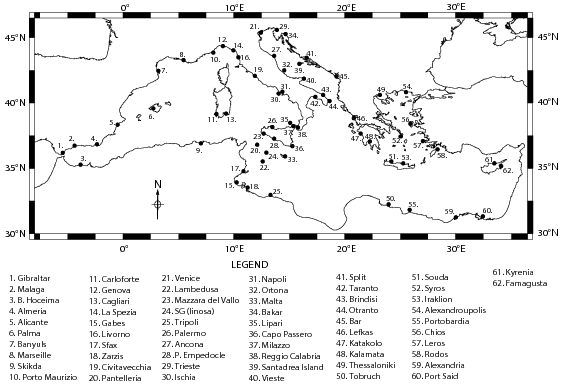
\includegraphics[width=0.6\textwidth]{./tides_in_the_Mediterranean_Sea/gauges.png}
\caption{Locations of 62 tide gauges in the Mediterranean Sea used to calculate the root mean square error.}
\end{figure}
\end{frame}


\begin{frame}
    \frametitle{Tides in the Mediterranean Sea - exercises}
\centering
\begin{itemize}
\item Consider the forcing tidal components contained in the netCDF file 'med.nc' (e.g. using ncview).
\item Examine the mesh features (e.g. open the '.msh' file in Gmsh).
\item Look at how to apply the forcing of different tidal components in the simulation.
\item Limit the error calculation by region, are the errors greater in some parts of the Mediterranean?
\end{itemize}
\end{frame}
